\chapter{Statistical Patterns in ODI Data}

\section{Run Rates}
One important factor in predicting who will win a game of cricket is run rate. This number tells the interested party how many runs are being
scored by the batting team per over. In this investigation, the decision to look at run rate per-ball rather than per-over in order to have
access to a greater wealth of data. 

The first plot, seen in figure 3.1 shows how the run-rate evolves over the course of an innings. The lefthand side shows the first innings, while on the right we have the second innings.
Immediately it is noticable that the first innings follows a logarithmic curve while the second innings eventually begins to follow an exponential curve.

\begin{figure}[h]
    \centering
    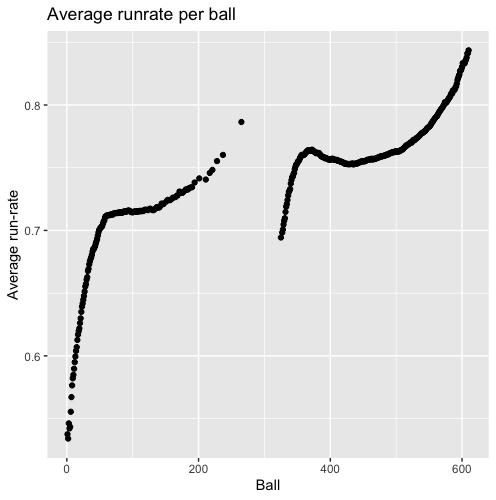
\includegraphics[scale=0.5]{figures/avgrrperball.png}
    \caption{Average run-rate per ball}
\end{figure}

The reason for the sharp increase in the first 60 balls of an innings is that this is the ``powerplay", when only a maximum of two fielders are allowed
in the outer field. This makes hitting high-scoring shots less risky for the batters. This drops off when the risk of this increases in the first innings, as the 
higher order batsmen aim to stay in for longer periods of time. Mathematically, one can see that the 